%=================================================================
% Standard LaTeX article — not journal-specific
%=================================================================
\documentclass[12pt,a4paper]{article}

\usepackage[utf8]{inputenc}
\usepackage[T1]{fontenc}
\usepackage[margin=2.5cm]{geometry}
\usepackage{amsmath,amssymb}
\usepackage{booktabs}
\usepackage{graphicx}
\usepackage{xurl}
\usepackage[colorlinks=true,linkcolor=blue,citecolor=blue,urlcolor=blue]{hyperref}
\usepackage[round,authoryear]{natbib}
\usepackage{threeparttable}
\usepackage[ruled,vlined,linesnumbered]{algorithm2e}
\usepackage{setspace}
\usepackage{authblk}
\usepackage{float}
\usepackage[protrusion=true,expansion=false]{microtype}

\onehalfspacing

\DeclareMathOperator*{\argmin}{arg\,min}

%=================================================================
% Title and authors
%=================================================================
\title{\textbf{Optimizing Pallet Configuration for Air Transport of Cut Flowers}}

\author[1]{Jaime Pesca%
  \thanks{Corresponding author: \href{mailto:jaime.e.pesca.s@gmail.com}{jaime.e.pesca.s@gmail.com}.
  ORCID: \href{https://orcid.org/0009-0003-8221-0924}{0009-0003-8221-0924}.}}
\author[2]{Edgar Gutierrez-Franco}
\author[2]{Christopher Mejia-Argueta}

\affil[1]{Faculty of Engineering, Universidad de La Sabana,
  Km.~7 Autopista Norte de Bogot\'{a}, Ch\'{i}a, Colombia}
\affil[2]{Center for Transportation and Logistics,
  Massachusetts Institute of Technology, Cambridge, MA~02142, USA}

\date{}

%=================================================================
\begin{document}
\maketitle

%=================================================================
\begin{abstract}
Air freight logistics represents a critical economic pillar for the
global cut flower industry, yet it faces significant challenges regarding
high transportation costs and perishable inventory management.
This study addresses the Air Cargo Loading Problem (ACLP) within the
specific context of a major South American flower supplier.
Unlike traditional offline optimisation methods, this research models
the loading process as an \emph{online} three-dimensional bin packing
problem, reflecting the real-world operational constraint where cargo
arrives sequentially with limited lookahead visibility.
We developed a Decision Support Model (DSM) utilising heuristic-based
packing strategies within the DeepPack3D framework, extending it from
single-bin evaluation to a realistic, heterogeneous multi-ULD
configuration matching the actual cargo layout of a Boeing~747-400F
aircraft (65~ULDs across four types).
The model was validated on historical data from 16~full charter flights
between Colombia/Ecuador and the United States.
The Bottom-Left (BL) heuristic achieved the highest mean volumetric
utilisation at 88.9\%, improving on the historical manual baseline of
84.0\% by a mean of 4.85~percentage points and by up to 8.4~percentage
points on individual flights.
The improvement translates into substantial additional cargo capacity
per flight and an estimated 8\% reduction in unit freight costs,
confirmed as statistically significant via a one-sided Wilcoxon
signed-rank test ($W=135$, $p<0.0001$).
\end{abstract}

\noindent\textbf{Keywords:} air cargo logistics; cut flower supply
chain; online 3D bin packing; heuristic optimisation; payload
maximisation; decision support model; Boeing 747-400F

\bigskip


%%%%%%%%%%%%%%%%%%%%%%%%%%%%%%%%%%%%%%%%%%
\section{Introduction}
\label{sec:intro}

The global floriculture market was valued at USD~64 billion in 2024 and
is projected to reach USD~119 billion by 2032, with cut flowers
representing a dominant 60\% of this total \citep{FloricultureMarket2025}.
This industry is fundamentally global and heavily reliant on exports.
The United States imports approximately 80\% of its flower consumption,
with two-thirds originating from Colombia and another one-sixth from
Ecuador \citep{Darras2021}.
This trade represents a significant economic pillar for these nations,
supporting thousands of jobs and contributing substantially to their
export revenues.

The cut flower supply chain is exceptionally complex, involving a
time-sensitive interaction between suppliers, growers, distributors, and
retailers who demand reliable, high-quality service for a highly
perishable product \citep{Paiva2024}.
A critical segment is the journey from greenhouse to airport --- a
24-hour window encompassing harvesting, grading, hydration, specialised
packaging, and refrigerated transport \citep{Sirisaranlak2017}.
At international auctions, even minor damage can reduce prices by
5--10\%, while more significant quality issues can slash prices by up
to 50\% \citep{Sirisaranlak2017}.

Air cargo transportation ensures rapid, safe delivery of high-value
perishable goods, making it essential for the floriculture industry
\citep{Hava2022}.
As of 2025, IATA forecasts a 5.8\% rise in air cargo volumes, reaching
72.5~million tonnes \citep{IATA2025}.
For South American flowers, the main air freight hubs are Bogot\'{a}
(Colombia) and Quito (Ecuador), with Miami (USA) as the principal
destination \citep{Fioravanti2022}.
Transportation costs can constitute 25--40\% of the final retail price
of flowers \citep{Button2020,Vega2008}, exposing companies to margin
pressure from volatile fuel prices and capacity constraints
\citep{Bonetti2022}.

Economic pressure drives the need for efficient packing of Unit Load
Devices (ULDs) --- air freight containers or pallets with specific size
and weight limits.
Effective packing improves transit efficiency, safety, and fuel usage,
reducing CO$_2$ emissions \citep{Zhao2023}.
The packing process must address geometry, payload, balance,
orientation, stackability, and stability --- collectively known as the
Air Cargo Loading Problem (ACLP) \citep{Chan2006a}, related to the
classic Bin Packing Problem (BPP) and Air Cargo Palletisation Problem
(ACPP) \citep{Paquay2018}.
Optimising the aircraft load factor is also critical for
sustainability: a 5\% increase in load factor raises fuel consumption
by approximately 1.3\% per available ton-mile
\citep{Brueckner2017,Queiroz2024}.

This study develops a DSM that formulates aircraft palletisation as an
online three-dimensional bin packing problem under realistic operational
constraints.
The methodology builds on the DeepPack3D framework \citep{Tsang2025},
extended to represent the full heterogeneous ULD set of a
Boeing~747-400F, using exclusively deterministic heuristic placement
policies within a sequential, aircraft-scale loading process.

\medskip\noindent
The main contributions of this study are:
\begin{enumerate}
  \item \textbf{Aircraft-scale online 3D bin packing model.}
        The DeepPack3D framework \citep{Tsang2025} is extended from
        single-bin evaluation to a heterogeneous 65-ULD configuration
        matching the actual cargo layout of a Boeing~747-400F, enabling
        aircraft-level utilisation measurement.

  \item \textbf{Industry-specific problem formulation.}
        The ACLP is formalised for the cut-flower industry, explicitly
        modelling the online, irreversible nature of conveyor-based
        palletisation, a gravitational stability constraint, and a
        dual-region curvature approximation for fuselage-adjacent
        containers.

  \item \textbf{Comparative evaluation on real operational data.}
        The DSM is validated on 16~full charter flights, demonstrating
        that the Bottom-Left heuristic improves on historical manual
        operations on 15 of 16~flights by up to 8.4~percentage points,
        with statistical significance confirmed via a Wilcoxon
        signed-rank test.

  \item \textbf{Quantified operational and environmental impact.}
        Volumetric gains are translated into an estimated 8\% reduction
        in unit freight costs and lower CO$_2$ intensity per kilogram
        of cargo.
\end{enumerate}

The remainder of this paper is organised as follows.
Section~\ref{sec:context} describes the case study context.
Section~\ref{sec:litreview} reviews the core literature on the BPP and
ACLP.
Section~\ref{sec:problem} formalises the problem mathematically.
Section~\ref{sec:method} details the solution methodology.
Section~\ref{sec:casestudy} presents the data and implementation.
Section~\ref{sec:results} discusses results.
Section~\ref{sec:conclusions} concludes.


%%%%%%%%%%%%%%%%%%%%%%%%%%%%%%%%%%%%%%%%%%
\section{Case Study Context}
\label{sec:context}

The sponsor company (SC) is a leading, vertically integrated cut flower
supplier with over 2{,}000~hectares of farmland in Colombia, Ecuador,
and Kenya.
The SC's supply chain begins with flowers harvested daily, sorted,
graded, and packed into boxes at the farm --- each labelled with an Air
Waybill (AWB) code for traceability.
These boxes are transported by refrigerated trucks to the nearest
airport, where airline staff build flight-specific ULDs via an
automated conveyor system.
The final arrangement of boxes is determined by experienced airline
personnel, relying on a first-come, first-loaded scheme that may not
produce optimal packings.

The general problem involves three interdependent decisions:
\begin{itemize}
  \item \textbf{Decision~1 --- Box Selection} (\emph{what to ship}):
        determining the mix of products to allocate to a specific
        flight.
  \item \textbf{Decision~2 --- Packing List} (\emph{how to load}):
        arranging the selected boxes within each ULD, defining the
        precise placement and orientation of every box.
  \item \textbf{Decision~3 --- ULD Allocation} (\emph{where to
        allocate}): determining the placement of each ULD within the
        aircraft's cargo hold to meet safety, operational, and balance
        requirements.
\end{itemize}

This study focuses exclusively on Decision~2.
Decisions~1 and~3 are treated as given inputs, consistent with the
SC's operational priorities and the scope of the DeepPack3D framework.
The US market is the SC's primary export destination, with Miami
airport as the main distribution hub.
The study covers two routes --- Quito to Miami (UIO-MIA) and
Bogot\'{a} to Miami (BOG-MIA) --- using Boeing~747-400F aircraft on
full charter flights.
Figure~\ref{fig:flow} illustrates the end-to-end operational flow from
farm dispatch to delivery.

\begin{figure}[htbp]
\centering
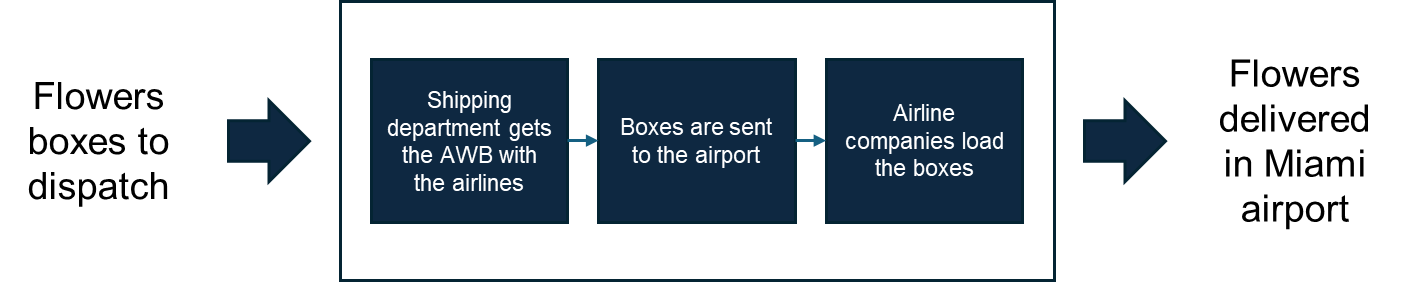
\includegraphics[width=0.88\textwidth]{figures/image1.png}
\caption{Operational flow of cut flower air freight: from farm dispatch
  through AWB generation, airport loading, and delivery at Miami
  International Airport.}
\label{fig:flow}
\end{figure}

The Boeing~747-400F configuration used in this study comprises
65~heterogeneous ULDs distributed across the main deck and lower holds
(Figure~\ref{fig:aircraft}).
Table~\ref{tab:ulds} lists the four ULD types and their internal
dimensions as modelled (width $\times$ height $\times$ depth, in
decimetres).

\begin{table}[htbp]
\caption{Boeing~747-400F ULD configuration used in the model.
  Dimensions are internal (W$\times$H$\times$D) in decimetres.}
\label{tab:ulds}
\centering
\begin{tabular}{@{}llrrrr@{}}
\toprule
\textbf{ULD type} & \textbf{Description}
  & \textbf{W (dm)} & \textbf{H (dm)} & \textbf{D (dm)}
  & \textbf{Count} \\
\midrule
M1   & Main-deck pallet        & 24 & 24 & 32 & 30 \\
M1H  & Lower-hold pallet slice &  6 & 12 & 32 & 23 \\
P6P  & Lower-hold pallet       & 24 & 16 & 32 &  9 \\
LD-1 & Lower-hold container    & 15 & 16 & 23 &  2 \\
Bulk & Bulk compartment        & 20 & 20 & 18 &  1 \\
\midrule
\multicolumn{5}{@{}l}{\textbf{Total}} & \textbf{65} \\
\bottomrule
\end{tabular}
\end{table}

\begin{figure}[htbp]
\centering
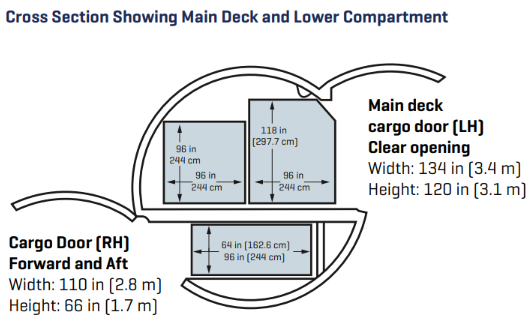
\includegraphics[width=0.72\textwidth]{figures/image2.png}
\caption{Cross-section of the Boeing~747-400F showing main deck and
  lower compartment ULD positions and door clearance dimensions.
  Source: Boeing Commercial Airplanes technical documentation.}
\label{fig:aircraft}
\end{figure}

To ground the modelling assumptions in Section~\ref{sec:limitations}
in actual practice, the authors conducted a site visit to the SC's
export cargo terminal at El Dorado International Airport (Bogot\'{a})
to observe the manual palletising process firsthand
(Figure~\ref{fig:visit}).
Boxes of heterogeneous heights are stacked and interlocked by hand
onto ULD pallets to conform to the contoured, sloped profile required
by the aircraft's lower-deck curvature, consistent with the automated
conveyor loading procedure described above.

\begin{figure}[htbp]
\centering
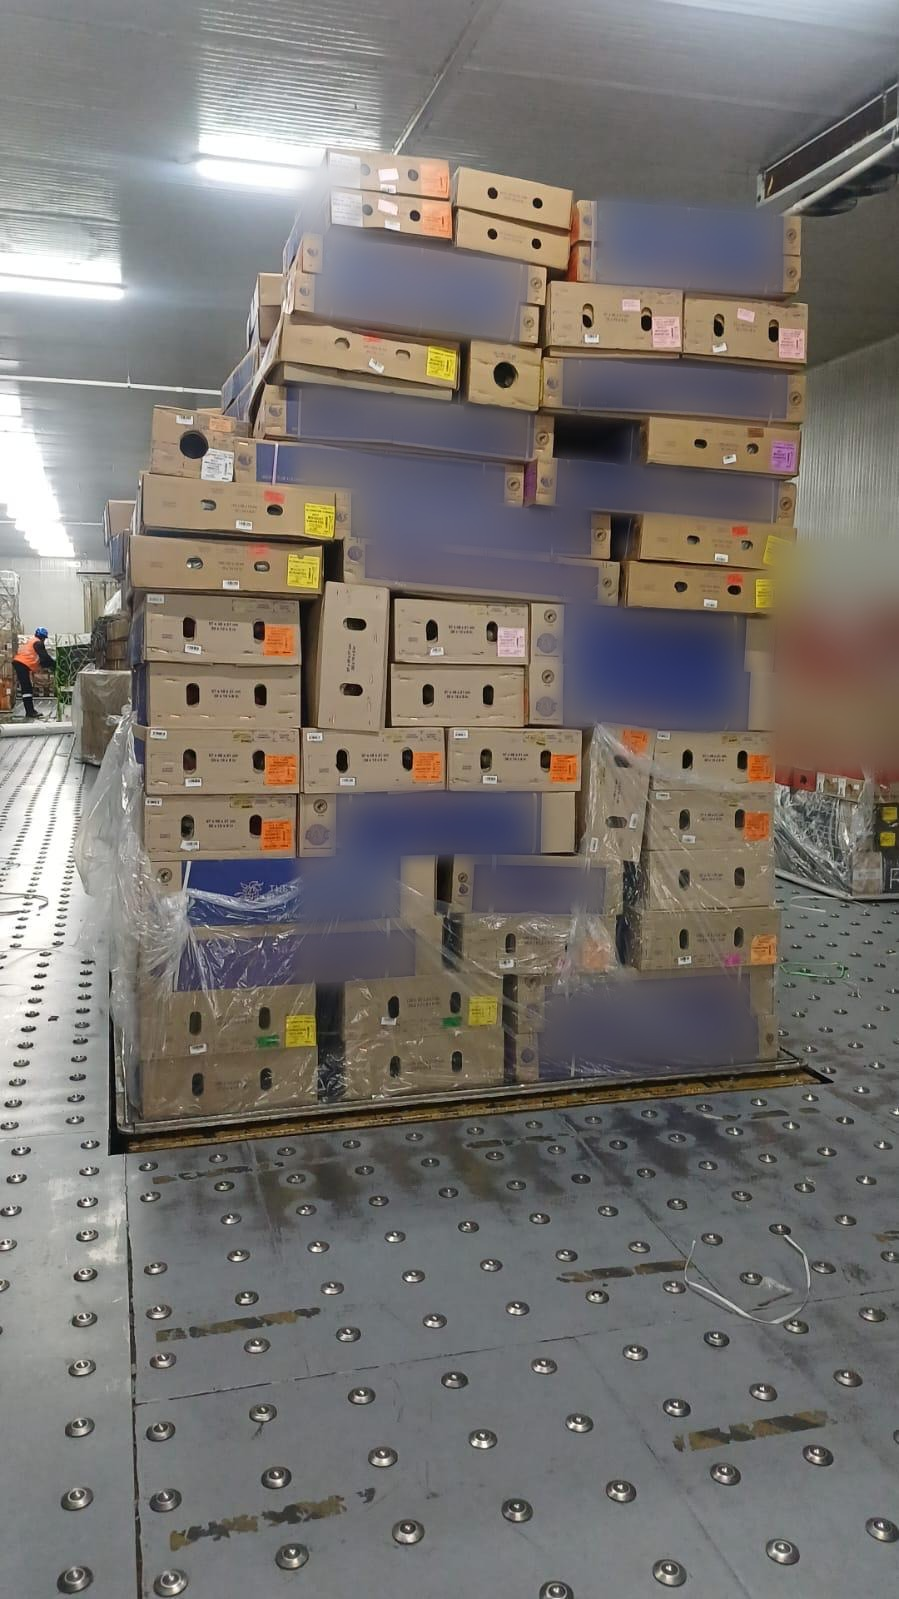
\includegraphics[width=0.62\textwidth]{figures/fig_site_visit.jpg}
\caption{Manual palletising of cut flower boxes observed during the
  site visit to the export cargo terminal at El Dorado International
  Airport (Bogot\'{a}). Boxes of varying heights are hand-stacked to
  conform to the ULD's contoured profile; brand markings have been
  obscured. Photograph by the authors.}
\label{fig:visit}
\end{figure}


%%%%%%%%%%%%%%%%%%%%%%%%%%%%%%%%%%%%%%%%%%
\section{Literature Review}
\label{sec:litreview}

This section reviews the foundational literature on the BPP and ACLP,
establishing the theoretical basis for this study.

\subsection{Bin Packing Problem}

The challenge of efficiently packing items into a container is a
long-standing problem in combinatorial optimisation.
\citet{George1980} introduced the first heuristic for the
three-dimensional container loading problem, filling a container layer
by layer and prioritising boxes that are harder to fit.
\citet{Martello2000} formalised the 3D-BPP as an NP-hard
combinatorial optimisation problem and provided the first exact
branch-and-bound algorithm alongside lower bounds that remain reference
benchmarks.
\citet{Bortfeldt2013} provide a comprehensive review of constraints
encountered in container loading --- including weight limits,
orientation restrictions, and fragility --- establishing the design
space within which practical algorithms operate.

\subsection{Sequential and Integrated Approaches for Air Cargo}

\citet{Chan2006a} propose a two-phase Decision Support Model: the
first phase applies Linear Programming (LP) for ULD selection, and
the second uses a heuristic to produce a detailed loading plan.
\citet{Paquay2018} present a two-phase constructive heuristic adapting
the Extreme Points method for a single ULD type, with post-processing
steps for weight balance and fragility constraints directly applicable
to the cut flower industry.
\citet{Zhao2023} propose a joint combinatorial optimisation of the
ACPP and the Aircraft Weight and Balance Problem via Integer Linear
Programming, achieving superior global optimisation for payload and
centre of gravity.

\subsection{Online Bin Packing and Heuristics}

A fundamental distinction separates offline methods --- requiring full
cargo knowledge prior to planning --- from online approaches where
decisions are made sequentially.
Offline methods such as \citet{Paquay2018} and \citet{Zhao2023} are
misaligned with the SC's operational context, where boxes arrive
continuously and placement decisions must be made irreversibly in real
time.

Constructive heuristics remain vital for online bin packing due to
computational efficiency and real-time adaptability \citep{Chazelle1983}.
\citet{Zhao2021} demonstrated that deep reinforcement learning can
learn effective online packing policies without manual rule design,
using a constrained action space that guarantees physical feasibility.
The DeepPack3D framework \citep{Tsang2025} extends this line of work
to multi-bin settings with bin replacement strategies, demonstrating
that well-tuned heuristics can rival more complex learning-based
agents in environments with limited lookahead.

Table~\ref{tab:litreview} compares the main references against criteria
most relevant to this study.

\begin{table}[htbp]
\caption{Comparison of main literature references against key criteria.}
\label{tab:litreview}
\centering
\begin{tabular}{@{}lccccc@{}}
\toprule
\textbf{Reference} & \textbf{Online} & \textbf{Multi-ULD}
  & \textbf{Industry-specific} & \textbf{Heuristic} & \textbf{RL} \\
\midrule
\citet{George1980}   & $\times$   & $\times$   & $\times$   & \checkmark & $\times$ \\
\citet{Martello2000} & $\times$   & $\times$   & $\times$   & \checkmark & $\times$ \\
\citet{Chan2006a}    & $\times$   & \checkmark & $\times$   & \checkmark & $\times$ \\
\citet{Paquay2018}   & $\times$   & \checkmark & $\times$   & \checkmark & $\times$ \\
\citet{Zhao2021}     & \checkmark & $\times$   & $\times$   & $\times$   & \checkmark \\
\citet{Zhao2023}     & $\times$   & \checkmark & $\times$   & $\times$   & $\times$ \\
\citet{Tsang2025}    & \checkmark & $\times$   & $\times$   & \checkmark & \checkmark \\
\textbf{This study}  & \checkmark & \checkmark & \checkmark & \checkmark & $\times$ \\
\bottomrule
\end{tabular}
\end{table}

Based on these criteria, the DeepPack3D framework \citep{Tsang2025}
is selected for alignment with the SC's online, sequential operational
reality.
While research in air cargo loading has advanced, few studies address
the specific commodity of cut flowers, whose unique traits ---
fragility, heterogeneous box sizes, and cold-chain requirements ---
are often overlooked.
This study addresses this gap by (i)~developing an industry-specific
model accounting for perishability and seasonality, (ii)~applying
online optimisation to the packing sequence and ULD configuration, and
(iii)~estimating CO$_2$ emissions alongside economic factors.


%%%%%%%%%%%%%%%%%%%%%%%%%%%%%%%%%%%%%%%%%%
\section{Problem Definition}
\label{sec:problem}

\subsection{Operational Problem Description}

The SC ships approximately 10{,}000~boxes daily, containing 100--500
SKUs for various clients.
Boxes arrive at the airport conveyor sequentially; placement decisions
are irreversible and must be made with limited visibility of future
arrivals.
The objective is to apply efficient local decision rules that maximise
space utilisation as the loading process unfolds, rather than compute
a globally optimal plan.

\subsection{Mathematical Formulation}
\label{sec:formulation}

Table~\ref{tab:notation} defines the notation used throughout.

\begin{table}[htbp]
\caption{Mathematical notation.}
\label{tab:notation}
\centering
\small
\begin{tabular}{@{}ll@{}}
\toprule
\textbf{Symbol} & \textbf{Description} \\
\midrule
\multicolumn{2}{@{}l}{\textit{Sets and indices}} \\
$N$               & Total number of boxes for a single flight \\
$M$               & Total number of ULDs on the aircraft ($M=65$) \\
$\mathcal{B} = (b_1,\ldots,b_N)$
  & Ordered box sequence (arrival order) \\
$\mathcal{U} = \{U_1,\ldots,U_M\}$
  & Set of ULDs (indexed by loading order) \\
$\mathcal{R}(b_i)$
  & Set of admissible axis-aligned rotations of box $b_i$ \\
\midrule
\multicolumn{2}{@{}l}{\textit{Box parameters}} \\
$(w_i, h_i, d_i)$ & Width, height, depth of box $b_i$ (original orientation) \\
$(w_i', h_i', d_i')$ & Effective dimensions after applying rotation $r_i$ \\
$m_i$             & Gross weight of box $b_i$ (kg) \\
$\mathrm{vol}(b_i)$ & Volume: $w_i h_i d_i$ \\
\midrule
\multicolumn{2}{@{}l}{\textit{ULD parameters}} \\
$(W_j, H_j, D_j)$ & Internal width, height, depth of $U_j$ \\
$C_j^w$           & Maximum weight capacity of $U_j$ (kg) \\
$\mathrm{Vol}(U_j)$ & Internal volume: $W_j H_j D_j$ \\
\midrule
\multicolumn{2}{@{}l}{\textit{Decision variables}} \\
$x_{ij} \in \{0,1\}$
  & 1 if box $b_i$ is assigned to ULD $U_j$ \\
$r_i \in \mathcal{R}(b_i)$
  & Selected rotation for $b_i$ \\
$(p_i^x, p_i^y, p_i^z) \in \mathbb{N}^3$
  & Placement origin of $b_i$ within its ULD \\
\midrule
\multicolumn{2}{@{}l}{\textit{State representation}} \\
$\mathcal{F}_j$
  & Set of free cuboid subspaces within $U_j$ \\
$\mathbf{H}_j \in \mathbb{N}^{D_j \times W_j}$
  & Height map: $\mathbf{H}_j(z,x)$ = stacking height at column $(x,z)$ \\
$k$               & Lookahead window size ($k=7$ in all experiments) \\
$\alpha$          & Minimum base-support fraction ($\alpha = 0.50$) \\
\bottomrule
\end{tabular}
\end{table}

\subsubsection{Objective Function}

The primary objective is to maximise mean volumetric utilisation
across all $M$ ULDs:
\begin{equation}
\label{eq:objective}
\text{maximise} \quad
\bar{U}_{\mathrm{vol}}
= \frac{1}{M} \sum_{j=1}^{M}
  \frac{\displaystyle\sum_{i=1}^{N} x_{ij}\, w_i' h_i' d_i'}
       {W_j H_j D_j}.
\end{equation}

\subsubsection{Constraints}

\textbf{C1 --- Unique assignment.}
Each box is assigned to at most one ULD:
\begin{equation}
\label{eq:c1}
\sum_{j=1}^{M} x_{ij} \leq 1, \quad \forall\, i.
\end{equation}

\textbf{C2 --- Geometric containment.}
If $x_{ij}=1$, the placed box must fit within $U_j$:
\begin{equation}
\label{eq:c2}
p_i^x + w_i' \leq W_j,\quad
p_i^y + h_i' \leq H_j,\quad
p_i^z + d_i' \leq D_j.
\end{equation}

\textbf{C3 --- Non-overlap.}
For all pairs $(b_i, b_{i'})$ assigned to the same ULD, the placed
cuboids must be disjoint:
\begin{equation}
\label{eq:c3}
\exists\,\delta\in\{x,y,z\} :
p_i^{\delta} + \ell_i^{(\delta)} \leq p_{i'}^{\delta}
\;\text{ or }\;
p_{i'}^{\delta} + \ell_{i'}^{(\delta)} \leq p_i^{\delta},
\end{equation}
where $\ell_i^{(x)}=w_i'$, $\ell_i^{(y)}=h_i'$, $\ell_i^{(z)}=d_i'$.

\textbf{C4 --- Gravitational stability.}
A placement at height $p_i^y$ is feasible only if at least fraction
$\alpha$ of the box's base footprint is supported at that height:
\begin{equation}
\label{eq:stability}
\frac{\bigl|\{(x,z)\in\mathrm{footprint}(b_i) :
              \mathbf{H}_j(z,x)=p_i^y\}\bigr|}
     {w_i' \cdot d_i'}
\;\geq\; \alpha = 0.50,
\end{equation}
where $\mathrm{footprint}(b_i) = [p_i^x, p_i^x+w_i') \times
[p_i^z, p_i^z+d_i')$ and the placement height is
$p_i^y = \max_{(x,z)\in\mathrm{footprint}(b_i)} \mathbf{H}_j(z,x)$.

\textbf{C5 --- ULD weight capacity (stated for completeness; not enforced).}
\begin{equation}
\label{eq:c5}
\sum_{i=1}^{N} x_{ij}\, m_i \leq C_j^w, \quad \forall\, j.
\end{equation}
This constraint completes the general ACLP formulation but is
\emph{not} implemented in the DSM: box weight $m_i$ is not tracked by
the online packing procedure (Section~\ref{sec:method}), so C5 is
never evaluated during placement.
The weight-based load factor is reported as a diagnostic from
historical AWB records (Table~\ref{tab:kpis}), not as an algorithmic
constraint; see Section~\ref{sec:limitations} for the rationale.

\textbf{C6 --- Online irreversibility.}
At step $t$, only the lookahead window
$\mathcal{W}_t = (b_t, \ldots, b_{\min(t+k-1,N)})$
is observable; placements cannot be revised once made.

\subsection{Scope and Assumptions}

Weight capacity (C5) is part of the general formulation above but is
not enforced by the implemented DSM, which tracks only box and ULD
geometry.
Volumetric efficiency is the primary limiting factor for cut flower
shipments, which are typically volume-constrained due to packaging
requirements and product fragility; this is confirmed empirically in
Section~\ref{sec:casestudy}, where the historical Weight-Based Load
Factor (73.7\%) is consistently below the Volume-Based Load Factor
(84.0\%).
Cargo arrives sequentially in arrival order; no global pre-sorting or
offline optimisation is applied.
Aircraft-level ULD allocation (Decision~3) is excluded from scope.


%%%%%%%%%%%%%%%%%%%%%%%%%%%%%%%%%%%%%%%%%%
\section{Solution Methodology}
\label{sec:method}

\subsection{Space Representation via Maximal Cuboid Partitioning}
\label{sec:space}

The free space inside each ULD $U_j$ is represented as a dynamic set
$\mathcal{F}_j$ of non-overlapping, axis-aligned \emph{maximal free
cuboids}.
At initialisation,
$\mathcal{F}_j = \{\mathrm{Cuboid}(0,0,0,W_j,H_j,D_j)\}$.
When a box is placed, every free cuboid intersecting the occupied
region is replaced by up to six maximal sub-cuboids
(Algorithm~\ref{alg:partition}), and dominated sub-cuboids are
discarded.
This avoids explicit voxelisation and remains tractable for the box
dimensions encountered in cut-flower operations.

A height map $\mathbf{H}_j \in \mathbb{N}^{D_j \times W_j}$ is
maintained in parallel.
After placing a box with effective dimensions $(w', h', d')$ at
origin $(p^x, p^y, p^z)$:
\begin{equation}
\label{eq:hmap}
\mathbf{H}_j(z, x) \leftarrow
\max\!\bigl(\mathbf{H}_j(z, x),\; p^y + h'\bigr),\quad
(x,z)\in[p^x,p^x\!+\!w')\times[p^z,p^z\!+\!d').
\end{equation}

\subsection{Heuristic Placement Policies}
\label{sec:heuristics}

Three deterministic placement heuristics are evaluated.
Each defines a scoring function $\sigma$ over the feasible placement
set $\mathcal{A}_t$ (Algorithm~\ref{alg:feasible}).
The placement with the minimum score is selected, with ties broken
lexicographically on subsequent score components.

For the area-based heuristics (BAF and BLSF), let $s$ denote the
hosting free cuboid, with $s_w$ and $s_h$ denoting its width
(x-dimension) and height (y-dimension) respectively.

\subsubsection{Bottom-Left (BL)}

The BL heuristic \citep{Chazelle1983} minimises the resulting occupied
height after placement, breaking ties by the rightward then forward
extent:
\begin{equation}
\label{eq:bl}
\sigma_{\mathrm{BL}}(p^x, p^y, p^z, w', h', d')
= \bigl(p^y + h',\; p^x + w',\; p^z + d'\bigr).
\end{equation}
By systematically minimising vertical growth, BL promotes compact,
layered packing patterns well suited to the rectangular geometry of
aircraft pallets.

\subsubsection{Best Area Fit (BAF)}

BAF selects the placement minimising the volume of the hosting free
cuboid $s$, preferring the tightest available space.
Ties are broken by the shorter horizontal/vertical residual
\citep{Tsang2025}:
\begin{equation}
\label{eq:baf}
\sigma_{\mathrm{BAF}}(s, w', h')
= \bigl(\mathrm{Vol}(s),\; \min(s_w - w',\, s_h - h')\bigr).
\end{equation}

\subsubsection{Best Long Side Fit (BLSF)}

BLSF minimises the residual along the longer dimension of the hosting
free cuboid \citep{Tsang2025}:
\begin{equation}
\label{eq:blsf}
\sigma_{\mathrm{BLSF}}(s, w', h')
= \max(s_w - w',\, s_h - h').
\end{equation}

\subsection{Multi-ULD Online Packing Procedure}
\label{sec:procedure}

Algorithm~\ref{alg:main} describes the complete sequential packing
procedure for a single charter flight.

\begin{algorithm}[htbp]
\SetAlgoLined\DontPrintSemicolon
\KwIn{$\mathcal{B}=(b_1,\ldots,b_N)$;\;
      $\mathcal{U}=(U_1,\ldots,U_M)$;\;
      heuristic $\mathcal{H}$;\; lookahead $k=7$;\; $\alpha=0.50$}
\KwOut{Packing plan $\Pi$;\; utilisation $\bar{U}_{\mathrm{vol}}$}
\ForEach{$U_j\in\mathcal{U}$}{
  $\mathcal{F}_j\leftarrow\{\mathrm{Cuboid}(0,0,0,W_j,H_j,D_j)\}$;\quad
  $\mathbf{H}_j\leftarrow\mathbf{0}^{D_j\times W_j}$\;}
$j\leftarrow 1$;\quad $t\leftarrow 1$\;
\While{$t\leq N$ \textbf{and} $j\leq M$}{
  $\mathcal{W}_t\leftarrow(b_t,\ldots,b_{\min(t+k-1,N)})$\tcp*{observe window}
  $\mathcal{A}_t\leftarrow
    \textsc{FeasiblePlacements}(\mathcal{W}_t,U_j,\mathcal{F}_j,\mathbf{H}_j,\alpha)$\;
  \uIf{$\mathcal{A}_t=\emptyset$}{
    $j\leftarrow j+1$\tcp*{current ULD full; open next}
  }
  \Else{
    $(b_i^*,r_i^*,\mathbf{p}^*)\leftarrow\argmin_{\mathcal{A}_t}\sigma_{\mathcal{H}}$\;
    Update $\mathcal{F}_j$ via \textsc{SpacePartition};\quad
    update $\mathbf{H}_j$;\quad record $(b_i^*,U_j)$ in $\Pi$;\quad
    $t\leftarrow t+1$\;
  }
}
$\bar{U}_{\mathrm{vol}}\leftarrow\dfrac{1}{M}
  \displaystyle\sum_{j=1}^{M}
  \frac{\sum_{(b_i,U_j)\in\Pi}\mathrm{vol}(b_i)}{\mathrm{Vol}(U_j)}$\;
\Return{$\Pi,\;\bar{U}_{\mathrm{vol}}$}
\caption{Multi-ULD Online 3D Bin Packing}
\label{alg:main}
\end{algorithm}

\begin{algorithm}[htbp]
\SetAlgoLined\DontPrintSemicolon
\KwIn{$\mathcal{W}_t$;\; $U_j$;\; $\mathcal{F}_j$;\;
      $\mathbf{H}_j$;\; $\alpha$}
\KwOut{$\mathcal{A}_t$}
$\mathcal{A}_t\leftarrow\emptyset$\;
\ForEach{$b_i\in\mathcal{W}_t$}{
  \ForEach{rotation $r\in\mathcal{R}(b_i)$, dims $(w',h',d')$}{
    \ForEach{$s\in\mathcal{F}_j$ with $s_w\geq w'$, $s_h\geq h'$,
             $s_d\geq d'$ and $s.\mathrm{top}=H_j$}{
      $p^y\leftarrow\max_{(x,z)\in\mathrm{footprint}}\mathbf{H}_j(z,x)$\;
      \If{$\dfrac{|\{(x,z)\in\mathrm{footprint}:\mathbf{H}_j(z,x)=p^y\}|}
                 {w'\cdot d'}\geq\alpha$
          \textbf{and} $p^y+h'\leq H_j$}{
        $\mathcal{A}_t\leftarrow
          \mathcal{A}_t\cup\{(b_i,r,(s^x,p^y,s^z),s)\}$\;
      }
    }
  }
}
\Return{$\mathcal{A}_t$}
\caption{\textsc{FeasiblePlacements}}
\label{alg:feasible}
\end{algorithm}

\begin{algorithm}[htbp]
\SetAlgoLined\DontPrintSemicolon
\KwIn{$\mathcal{F}$;\; placed cuboid $c$}
\KwOut{$\mathcal{F}'$}
$\mathcal{F}'\leftarrow\emptyset$;\quad $\mathcal{F}_\mathrm{new}\leftarrow\emptyset$\;
\ForEach{$s\in\mathcal{F}$}{
  \uIf{$s$ intersects $c$}{
    $\mathcal{F}_\mathrm{new}\leftarrow
      \mathcal{F}_\mathrm{new}\cup\textsc{MaximalSplit}(s,c)$\;
  }
  \Else{
    $\mathcal{F}'\leftarrow\mathcal{F}'\cup\{s\}$\;
  }
}
\ForEach{$s\in\mathcal{F}_\mathrm{new}$ not dominated by any
  $s'\in\mathcal{F}'\cup\mathcal{F}_\mathrm{new}$}{
  $\mathcal{F}'\leftarrow\mathcal{F}'\cup\{s\}$\;
}
\Return{$\mathcal{F}'$}
\caption{\textsc{SpacePartition}: maximal-cuboid decomposition}
\label{alg:partition}
\end{algorithm}

\subsection{Practical Adaptations and Aircraft-Specific Modelling}
\label{sec:adaptations}

The original DeepPack3D formulation assumes a single, fixed-size bin.
This study extends the framework to a finite, sequential multi-bin
configuration matching the actual cargo positions of a Boeing~747-400F.
ULDs are opened and filled in a predefined operational order; when no
feasible placement exists for any lookahead box, the current ULD is
closed and the next one opened (Algorithm~\ref{alg:main}, line 6).

The key implementation change is the \texttt{bin\_sizes} parameter
introduced in \texttt{env.py}: a list of $(W_j, H_j, D_j)$ tuples,
one per ULD, enabling the environment to open each successive bin with
the correct heterogeneous dimensions (Table~\ref{tab:ulds}).
When \texttt{bin\_sizes} is \texttt{None}, all bins share a common
size, recovering the original single-type behaviour.
All experiments use a lookahead window of $k=7$ boxes.

Although all ULDs are currently modelled as rectangular
parallelepipeds, real aircraft containers exhibit fuselage curvature.
The model architecture supports a dual-region decomposition ---
separating a reduced-height fuselage-adjacent region from a full-height
central region --- providing a pathway toward increasingly realistic
geometry-aware models.

\subsection{Key Performance Indicators}

Table~\ref{tab:kpis} defines the KPIs used to evaluate the DSM.

\begin{table}[htbp]
\caption{Key Performance Indicators for DSM evaluation.}
\label{tab:kpis}
\centering
\begin{tabular}{@{}lll@{}}
\toprule
\textbf{KPI} & \textbf{Formula} & \textbf{Unit} \\
\midrule
Volume-Based Load Factor &
  $\sum_i\mathrm{vol}(b_i)\,/\,\sum_j\mathrm{Vol}(U_j)$ & \% \\[3pt]
Weight-Based Load Factor &
  $\sum_i m_i\,/\,\sum_j C_j^w$ & \% \\[3pt]
Additional boxes packed &
  $|\Pi_\mathrm{DSM}|-|\Pi_\mathrm{hist}|$ & units \\[3pt]
CO$_2$ per kg cargo &
  $E_\mathrm{flight}\,/\,\sum_i m_i$ & kg\,CO$_2$/kg \\
\bottomrule
\end{tabular}
\end{table}


%%%%%%%%%%%%%%%%%%%%%%%%%%%%%%%%%%%%%%%%%%
\section{Case Study}
\label{sec:casestudy}

\subsection{Dataset Description}

The SC provided historical air freight data from January 2024 to
May 2025, comprising: (i)~flight-level records for the 16~analysed
charter flights and their AWBs; (ii)~AWB-level data including gross
weight, volumetric weight, and box quantities; and
(iii)~shipment-level details with box dimensions, flower types, and
customer information.
Data validation included cross-referencing AWB weights with airline
charge reports and outlier analysis on box dimensions, validated
during site visits to the cargo area at El Dorado Airport
(Bogot\'{a}).

Table~\ref{tab:baseline} presents baseline KPIs for the 16~flights.
The average Volume-Based Load Factor of 84\% indicates that
approximately 16\% of available volume is unused per flight.
The lower Weight-Based Load Factor of 73.7\% confirms that shipments
are volume-constrained --- low-density flower boxes fill space before
reaching weight capacity.

\begin{table}[htbp]
\caption{Baseline KPIs across 16 historical charter flights.}
\label{tab:baseline}
\centering
\begin{tabular}{@{}lrr@{}}
\toprule
\textbf{KPI} & \textbf{Mean} & \textbf{Range} \\
\midrule
Volume-Based Load Factor & 84.0\,\% & 81\,\%--89\,\% \\
Weight-Based Load Factor & 73.7\,\% & --- \\
CO$_2$ per kg cargo (benchmark) & 2.84\,kg/kg & --- \\
\bottomrule
\end{tabular}
\end{table}

\subsection{Box Size Distribution}

Across the 16~flights, 68~distinct box sizes were identified.
Of these, 15~references (22\% of box types) account for 90.8\% of
the total shipped volume.
During preprocessing, 53~low-frequency box sizes ($<$0.5\% of total
volume) were excluded from the model inputs; a sensitivity analysis
confirmed this exclusion does not significantly alter density patterns.
Figure~\ref{fig:pareto} illustrates the Pareto distribution.

\begin{figure}[htbp]
\centering
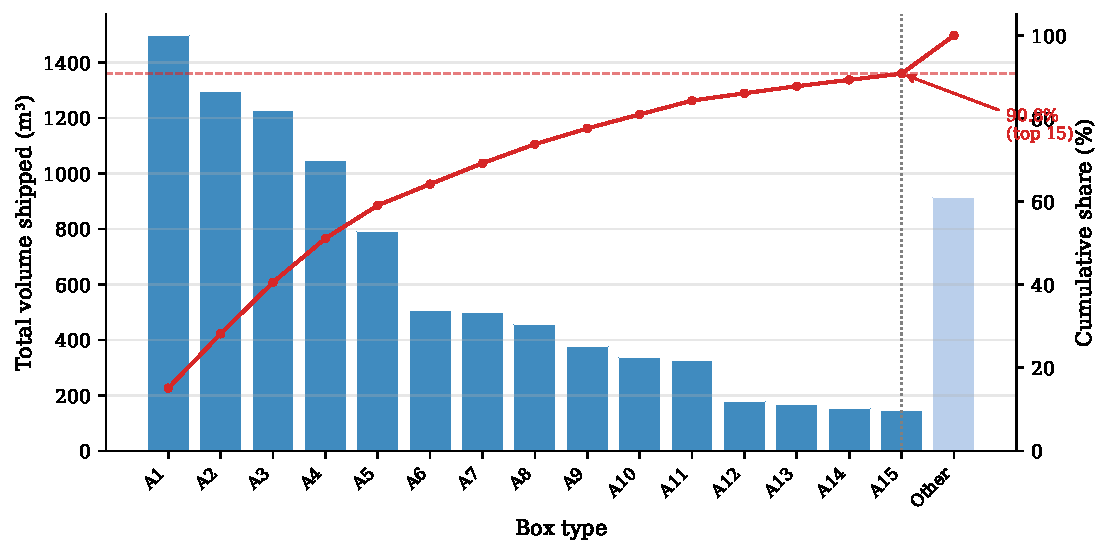
\includegraphics[width=\textwidth]{figures/fig_pareto.pdf}
\caption{Pareto distribution of box types by total volume shipped
  across 16 charter flights (January 2024 -- May 2025). The top~15
  box types (A1--A15) account for 90.8\% of total volume; remaining
  types (shaded) are excluded from model inputs.}
\label{fig:pareto}
\end{figure}

\subsection{Implementation Details}

All experiments used Python 3.10, TensorFlow 2.10.0, and NumPy 1.26.4.
Only the heuristic-based placement policies of the DeepPack3D
framework were activated; reinforcement learning components were not
used.
The lookahead window was set to $k=7$ boxes for all heuristics, and
the ULD configuration followed Table~\ref{tab:ulds} (65~ULDs, 4
types, total internal volume $\approx$735\,dm$^3$ per ULD type
summed to $\approx$735\,m$^3$ for the aircraft).

\subsection{Experimental Design}

For each of the 16~flights, the historical shipment was taken as the
baseline.
An additional set of 2{,}000~boxes was randomly sampled from the
remaining box population of that flight, preserving the empirical
distribution of box dimensions, to evaluate the model's ability to
exploit unused capacity.
The DSM receives all boxes (historical plus sampled) in a single
sequential stream; volumetric utilisation is measured over all 65~ULDs.


%%%%%%%%%%%%%%%%%%%%%%%%%%%%%%%%%%%%%%%%%%
\section{Results and Discussion}
\label{sec:results}

\subsection{Benchmarking Against the Historical Baseline}

The 16~historical flights exhibit volumetric utilisation of
81.1\%--88.6\% with a mean of 84.0\%, reflecting variation in cargo
composition and manual planning decisions.

\subsection{DSM Packing Performance}

The BL heuristic achieves a mean volumetric utilisation of 88.9\%
across all 16~flights, an improvement of $+$4.85~percentage points
(pp) over the historical baseline.
Per-flight BL utilisation ranges from 83.3\% to 90.8\%.
On 15 of 16~flights, BL outperforms the historical baseline by
2.2~pp to 8.4~pp; on one flight (F12), BL slightly underperforms the
historical value by 1.9~pp, which contributes to BL's lower standard
deviation relative to the historical spread.
Figure~\ref{fig:perflight} shows per-flight utilisation for all
methods.

\begin{figure}[htbp]
\centering
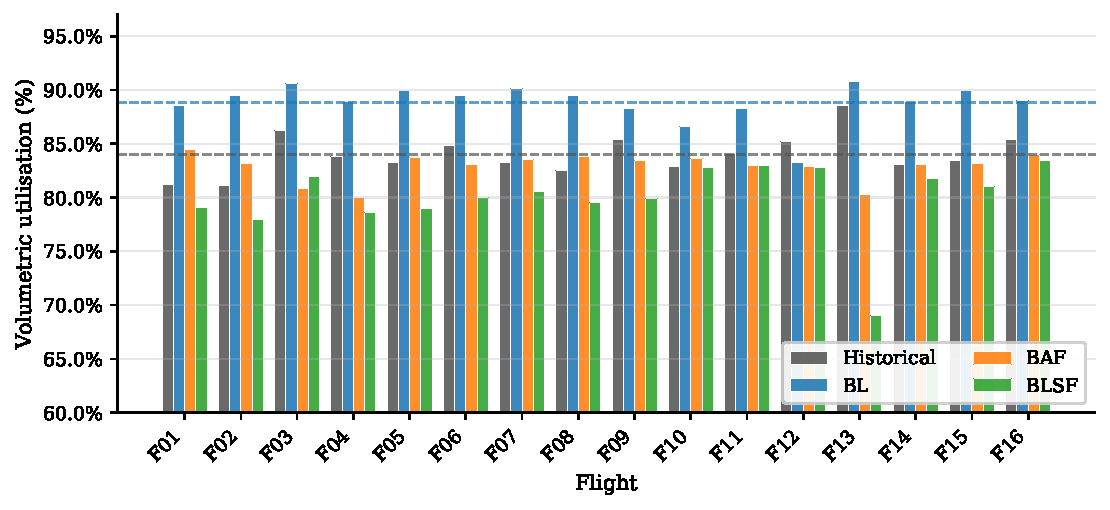
\includegraphics[width=\textwidth]{figures/fig_per_flight.pdf}
\caption{Per-flight volumetric utilisation (\%) across 16 charter
  flights for the historical baseline and the three heuristic
  policies. Dashed horizontal lines indicate the cross-flight mean
  for Historical (grey) and BL (blue).}
\label{fig:perflight}
\end{figure}

\subsection{Comparative Analysis of Heuristic Policies}

Table~\ref{tab:comparative} summarises comparative performance across
all flights.

\begin{table}[htbp]
\caption{Comparative volumetric utilisation across 16 charter flights
  (values in \%). $\Delta$\,mean = improvement over historical
  baseline (percentage points, pp). Statistical significance assessed
  via one-sided Wilcoxon signed-rank test ($n=16$, $\alpha=0.05$).}
\label{tab:comparative}
\begin{threeparttable}
\centering
\begin{tabular}{@{}lrrrrrrc@{}}
\toprule
\textbf{Method} & \textbf{Mean} & \textbf{Std} & \textbf{Min}
  & \textbf{Max} & \textbf{Median} & \textbf{$\Delta$ mean (pp)}
  & \textbf{$p$-value} \\
\midrule
Historical (baseline)
  & 84.02 & 1.90 & 81.10 & 88.60 & 83.60
  & --- & --- \\
Bottom-Left (BL)
  & \textbf{88.87} & 1.81 & 83.30 & 90.80 & 89.25
  & $+$4.85 & $<$0.0001\tnote{***} \\
Best Area Fit (BAF)
  & 82.88 & 1.32 & 80.00 & 84.50 & 83.20
  & $-$1.14 & 0.909\tnote{ns} \\
Best Long Side Fit (BLSF)
  & 80.03 & 3.40 & 69.00 & 83.40 & 80.30
  & $-$3.99 & 1.000\tnote{ns} \\
\bottomrule
\end{tabular}
\begin{tablenotes}
  \small
  \item[***] $p < 0.001$;\quad ns = not significant ($p > 0.05$).
  \item One-sided test: $H_0$: median difference $= 0$;\;
        $H_1$: heuristic $>$ baseline.
  \item Bold indicates best-performing heuristic.
\end{tablenotes}
\end{threeparttable}
\end{table}

\begin{figure}[htbp]
\centering
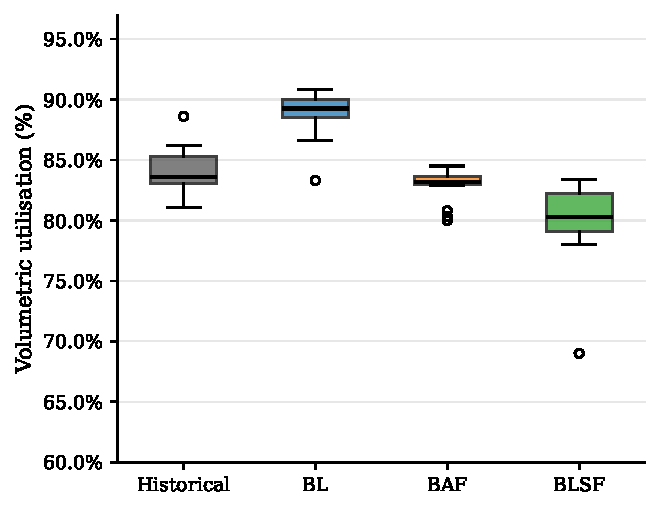
\includegraphics[width=0.62\textwidth]{figures/fig_boxplot.pdf}
\caption{Box plots of volumetric utilisation (\%) across 16 charter
  flights for each packing method. Circles denote outliers beyond
  1.5~IQR. The BL heuristic achieves a consistently higher median
  than the historical baseline; BAF and BLSF underperform the
  baseline on average.}
\label{fig:boxplot}
\end{figure}

BL's performance is driven by its lexicographic placement criterion:
minimising stacking height before lateral extent, which naturally
constructs dense base layers, fills corners efficiently, and limits
vertical fragmentation --- characteristics well-suited to the
geometry of Boeing~747-400F pallets and the dimensional variability
of cut flower boxes.

BAF and BLSF, by contrast, underperform relative to the historical
baseline on average ($-$1.14~pp and $-$3.99~pp, respectively).
BAF's area-fit criterion tends to fragment available space into many
small residuals, reducing packing efficiency for heterogeneous
box-size distributions.
BLSF shows the most severe degradation: its long-side minimisation
criterion is sensitive to box orientation and produced a 69.0\%
utilisation on one flight --- below the historical floor --- leading
to an overall mean of 80.03\%.

\subsection{Statistical Significance}

A one-sided Wilcoxon signed-rank test \citep{Wilcoxon1945} was
applied to paired differences between each heuristic and the
historical baseline across the 16~flights
($H_0$: equal median utilisation; $H_1$: heuristic $>$ baseline).
The non-parametric test is preferred given the small sample size
($n=16$) and the bounded nature of the utilisation metric.
Results (Table~\ref{tab:comparative}) show that BL yields a
statistically significant improvement over the historical baseline
($W = 135$, $p < 0.0001$, $\alpha = 0.05$).
BAF and BLSF do not improve significantly over the baseline
($p = 0.909$ and $p = 1.000$, respectively), consistent with their
negative mean differences.
These findings indicate that BL is the only heuristic among those
evaluated that reliably outperforms current manual palletisation
practice under the conditions observed in the dataset.

\subsection{Financial and Environmental Impact}

Higher load factors achieved by BL directly reduce per-box freight
costs.
Higher load factors also reduce CO$_2$ intensity below the benchmark
of 2.84\,kg\,CO$_2$/kg, since the same flight-level emissions are
distributed over a greater cargo weight
\citep{Baxter2020,Queiroz2024}.
The ICAO Carbon Emissions Calculator \citep{ICAO2025} estimates that
increasing payload by 8\% on a Boeing~747-400F route translates to a
reduction of approximately 0.18\,kg\,CO$_2$ per additional kilogram
of cargo transported.


%%%%%%%%%%%%%%%%%%%%%%%%%%%%%%%%%%%%%%%%%%
\section{Conclusions}
\label{sec:conclusions}

This study developed and evaluated a DSM for the palletisation of cut
flower shipments in full-charter air freight operations, formulated as
an online three-dimensional bin packing problem.
By embedding heuristic-based packing policies within an aircraft-scale
simulation framework, the DSM demonstrated that substantial
improvements in volumetric utilisation can be achieved without
learning-based optimisation.
When applied to real data from Boeing~747-400F charter flights, the
Bottom-Left heuristic improved on historical manual palletisation in
15 of 16~flights, with per-flight gains of 2.2~pp to 8.4~pp and a
mean improvement of $+$4.85~pp, statistically significant via
Wilcoxon test ($p<0.0001$).

The key contribution is the adaptation of an academic online 3D BPP
framework to a realistic multi-ULD aircraft environment, with explicit
representation of the finite heterogeneous 65-ULD set and a
sequential loading routine consistent with airline procedures.

\subsection{Limitations}
\label{sec:limitations}

First, validation is limited to 16~charter flights from a single
company; generalisation to other carriers, routes, or aircraft has
not been tested.
Second, all ULDs are modelled as rectangular parallelepipeds; because
this approximation neglects fuselage curvature, it tends to
\emph{underestimate}, rather than overestimate, the usable volume in
lower-deck positions.
Third, the model is purely volume-driven: neither box weight $m_i$
nor ULD weight capacity $C_j^w$ is tracked by the implementation, so
constraint C5 (Section~\ref{sec:formulation}) is stated for
completeness but never enforced.
This reflects the operational reality of the cargo, confirmed through
an on-site visit (Figure~\ref{fig:visit}): cut flower boxes are
consistently well below the aircraft's weight limits, so weight
capacity is non-binding.
However, the volume-only formulation does not encode other operational
constraints such as box fragility, airflow clearances, and
customer-specific priorities, which should be incorporated in future
work.
Finally, preliminary experiments with the reinforcement learning
components of DeepPack3D did not achieve results competitive with the
heuristic policies at the scale of the full 65-ULD configuration; a
more thorough RL comparison is reserved for future work.

\subsection{Future Work}
\label{sec:future}

Future directions include: (i)~refined curvature modelling through
detailed fuselage height profiles; (ii)~physical validation of
admissible box orientations for fragile cargo; (iii)~hybrid
heuristic-learning approaches that adaptively select placement rules;
and (iv)~full RL training within the extended multi-ULD aircraft
framework.


%%%%%%%%%%%%%%%%%%%%%%%%%%%%%%%%%%%%%%%%%%
\section*{Acknowledgements}

\textbf{Author contributions:}
Conceptualisation, J.P., E.G.-F.\ and C.M.-A.;
methodology, J.P.\ and E.G.-F.;
software, J.P.;
formal analysis, J.P.;
data curation, J.P.\ and C.M.-A.;
writing --- original draft, J.P.;
writing --- review and editing, J.P., E.G.-F.\ and C.M.-A.;
supervision, E.G.-F.

\textbf{Funding:} This research received no external funding.

\textbf{Data availability:}
The historical flight dataset was provided by the sponsor company
under a confidentiality agreement and is not publicly available.
The implementation code is available at
\url{https://github.com/JaimePesca/optimizing_pallet_configuration}.

\textbf{Conflicts of interest:} The authors declare no conflicts of
interest.


%%%%%%%%%%%%%%%%%%%%%%%%%%%%%%%%%%%%%%%%%%
\bibliographystyle{plainnat}
\begin{thebibliography}{99}

\bibitem[Floriculture Market(2025)]{FloricultureMarket2025}
Floriculture Market: Global Industry Analysis and Forecast (2025--2032).
\textit{Maximize Market Research} \textbf{2025}.
\url{https://www.maximizemarketresearch.com/market-report/global-floriculture-market/23982/}
(accessed 16 August 2025).

\bibitem[Darras(2021)]{Darras2021}
Darras, A. Overview of the dynamic role of specialty cut flowers in
the international cut flower market.
\textit{Horticulturae} \textbf{2021}, \textit{7}, 51.
\url{https://doi.org/10.3390/horticulturae7030051}

\bibitem[Paiva et al.(2024)]{Paiva2024}
Paiva, P.D.O.; Castro, A.C.R.; Geest, A.P.S.L.V.D.; Vieira, G.F.R.;
Hummel, M.; Lopes, H.D.S.; Costa, J.L.D.S.
Diagnosis of the production chain of flowers, turfgrass, and
ornamental plants.
\textit{Ornamental Horticulture} \textbf{2024}, \textit{30}, e242792.
\url{https://doi.org/10.1590/2447-536x.v30.e242792}

\bibitem[Sirisaranlak(2017)]{Sirisaranlak2017}
Sirisaranlak, P. The cool supply chain management for cut flowers.
In \textit{Proceedings of the 8th International Science, Social
Science, Engineering and Energy Conference}, Thailand, 2017.

\bibitem[Hava(2022)]{Hava2022}
Hava, H. Evaluation of the effects of air cargo transportation on
global competitiveness.
\textit{Journal of Aviation} \textbf{2022}, 206--217.

\bibitem[IATA(2025)]{IATA2025}
IATA. \textit{2025 Vision for the Future of Air Cargo Facilities};
IATA: Montreal, Canada, 2025.

\bibitem[Fioravanti et al.(2022)]{Fioravanti2022}
Fioravanti, R.; Ansaldo, M.; Caf\'{e}, E.; Fageda, X.; Ricover, A.
El transporte de carga a\'{e}rea en Am\'{e}rica Latina y el Caribe.
\textit{BID} \textbf{2022}.

\bibitem[Button(2020)]{Button2020}
Button, K. The economics of Africa's floriculture air-cargo supply
chain.
\textit{Journal of Transport Geography} \textbf{2020}, \textit{86},
102789.
\url{https://doi.org/10.1016/j.jtrangeo.2020.102789}

\bibitem[Vega(2008)]{Vega2008}
Vega, H. The transportation costs of fresh flowers: A comparison
between Ecuador and major exporting countries.
\textit{Inter-American Development Bank} \textbf{2008}.
\url{https://doi.org/10.18235/0011060}

\bibitem[Bonetti and Zidziunas(2022)]{Bonetti2022}
Bonetti, J.; Zidziunas, A. Air freight impact on the Colombian flower
industry.
\textit{MBA~661~I: International Trade and Investment}, 2022.

\bibitem[Zhao et al.(2023)]{Zhao2023}
Zhao, X.; Dong, Y.; Zuo, L. A combinatorial optimization approach for
air cargo palletization and aircraft loading.
\textit{Mathematics} \textbf{2023}, \textit{11}, 2798.
\url{https://doi.org/10.3390/math11132798}

\bibitem[Chan et al.(2006)]{Chan2006a}
Chan, F.T.S.; Bhagwat, R.; Kumar, N.; Tiwari, M.K.; Lam, P.
Development of a decision support system for air-cargo pallets loading
problem.
\textit{Expert Systems with Applications} \textbf{2006}, \textit{31},
472--485.
\url{https://doi.org/10.1016/j.eswa.2005.09.057}

\bibitem[Paquay et al.(2018)]{Paquay2018}
Paquay, C.; Limbourg, S.; Schyns, M. A tailored two-phase
constructive heuristic for the three-dimensional Multiple Bin Size
Bin Packing Problem.
\textit{European Journal of Operational Research} \textbf{2018},
\textit{267}, 52--64.
\url{https://doi.org/10.1016/j.ejor.2017.11.010}

\bibitem[Brueckner and Abreu(2017)]{Brueckner2017}
Brueckner, J.K.; Abreu, C. Airline fuel usage and carbon emissions:
Determining factors.
\textit{Journal of Air Transport Management} \textbf{2017},
\textit{62}, 10--17.
\url{https://doi.org/10.1016/j.jairtraman.2017.01.004}

\bibitem[Queiroz J\'{u}nior et al.(2024)]{Queiroz2024}
Queiroz J\'{u}nior, H.D.S.; Celestino, M.A.D.S.; De Souza, C.F.F.;
Falc\~{a}o, V.A.; Camioto, F.D.C. CO$_2$ emissions in air transport.
\textit{Transportation Research Record} \textbf{2024}, \textit{2678},
872--883.
\url{https://doi.org/10.1177/03611981231193407}

\bibitem[Tsang et al.(2025)]{Tsang2025}
Tsang, Y.P.; Mo, D.Y.; Chung, K.T.; Lee, C.K.M. A deep reinforcement
learning approach for online and concurrent 3D bin packing
optimisation with bin replacement strategies.
\textit{Computers in Industry} \textbf{2025}, \textit{164}, 104202.
\url{https://doi.org/10.1016/j.compind.2024.104202}

\bibitem[George and Robinson(1980)]{George1980}
George, J.A.; Robinson, D.F. A heuristic for packing boxes into a
container.
\textit{Computers \& Operations Research} \textbf{1980}, \textit{7},
147--156.
\url{https://doi.org/10.1016/0305-0548(80)90001-5}

\bibitem[Martello et al.(2000)]{Martello2000}
Martello, S.; Pisinger, D.; Vigo, D. The three-dimensional bin packing
problem.
\textit{Operations Research} \textbf{2000}, \textit{48}, 256--267.
\url{https://doi.org/10.1287/opre.48.2.256.12386}

\bibitem[Bortfeldt and W\"{a}scher(2013)]{Bortfeldt2013}
Bortfeldt, A.; W\"{a}scher, G. Constraints in container loading --- A
state-of-the-art review.
\textit{European Journal of Operational Research} \textbf{2013},
\textit{229}, 1--20.
\url{https://doi.org/10.1016/j.ejor.2012.12.006}

\bibitem[Chazelle(1983)]{Chazelle1983}
Chazelle, B. The bottom-left bin-packing heuristic: An efficient
implementation.
\textit{IEEE Transactions on Computers} \textbf{1983}, \textit{C-32},
697--707.

\bibitem[Zhao et al.(2021)]{Zhao2021}
Zhao, H.; She, Q.; Zhu, C.; Yang, Y.; Xu, K. Online 3D bin packing
with constrained deep reinforcement learning.
In \textit{Proceedings of the 35th AAAI Conference on Artificial
Intelligence (AAAI-21)};
AAAI Press: Palo Alto, CA, USA, 2021; pp.~741--749.
\url{https://doi.org/10.1609/aaai.v35i1.16155}

\bibitem[Wilcoxon(1945)]{Wilcoxon1945}
Wilcoxon, F. Individual comparisons by ranking methods.
\textit{Biometrics Bulletin} \textbf{1945}, \textit{1}, 80--83.
\url{https://doi.org/10.2307/3001968}

\bibitem[Baxter(2020)]{Baxter2020}
Baxter, G. Assessing the carbon footprint of a dedicated all-cargo
airline: The case of Cargolux International Airlines.
\textit{Journal of Urban and Environmental Engineering} \textbf{2020},
\textit{14}, 204--217.
\url{https://doi.org/10.4090/juee.2020.v14n2.204217}

\bibitem[ICAO(2025)]{ICAO2025}
ICAO. ICAO Carbon Emissions Calculator, 2025.
\url{https://www.icao.int/environmental-protection/environmental-tools/icec}

\end{thebibliography}

\end{document}
